\documentclass{beamer}

\usetheme{simple}

\usepackage{caption}
\usepackage{xcolor}
\usepackage{fancyvrb}
\usepackage{ulem}
\usetikzlibrary{positioning,calc,automata}

\title{CSC363 Tutorial \#3}
\subtitle{CE sets, Normal Form Theorem...}
\date{February 02, 2022}
\institute{}

\newcommand{\N}{\mathbb N}

\setwatermark{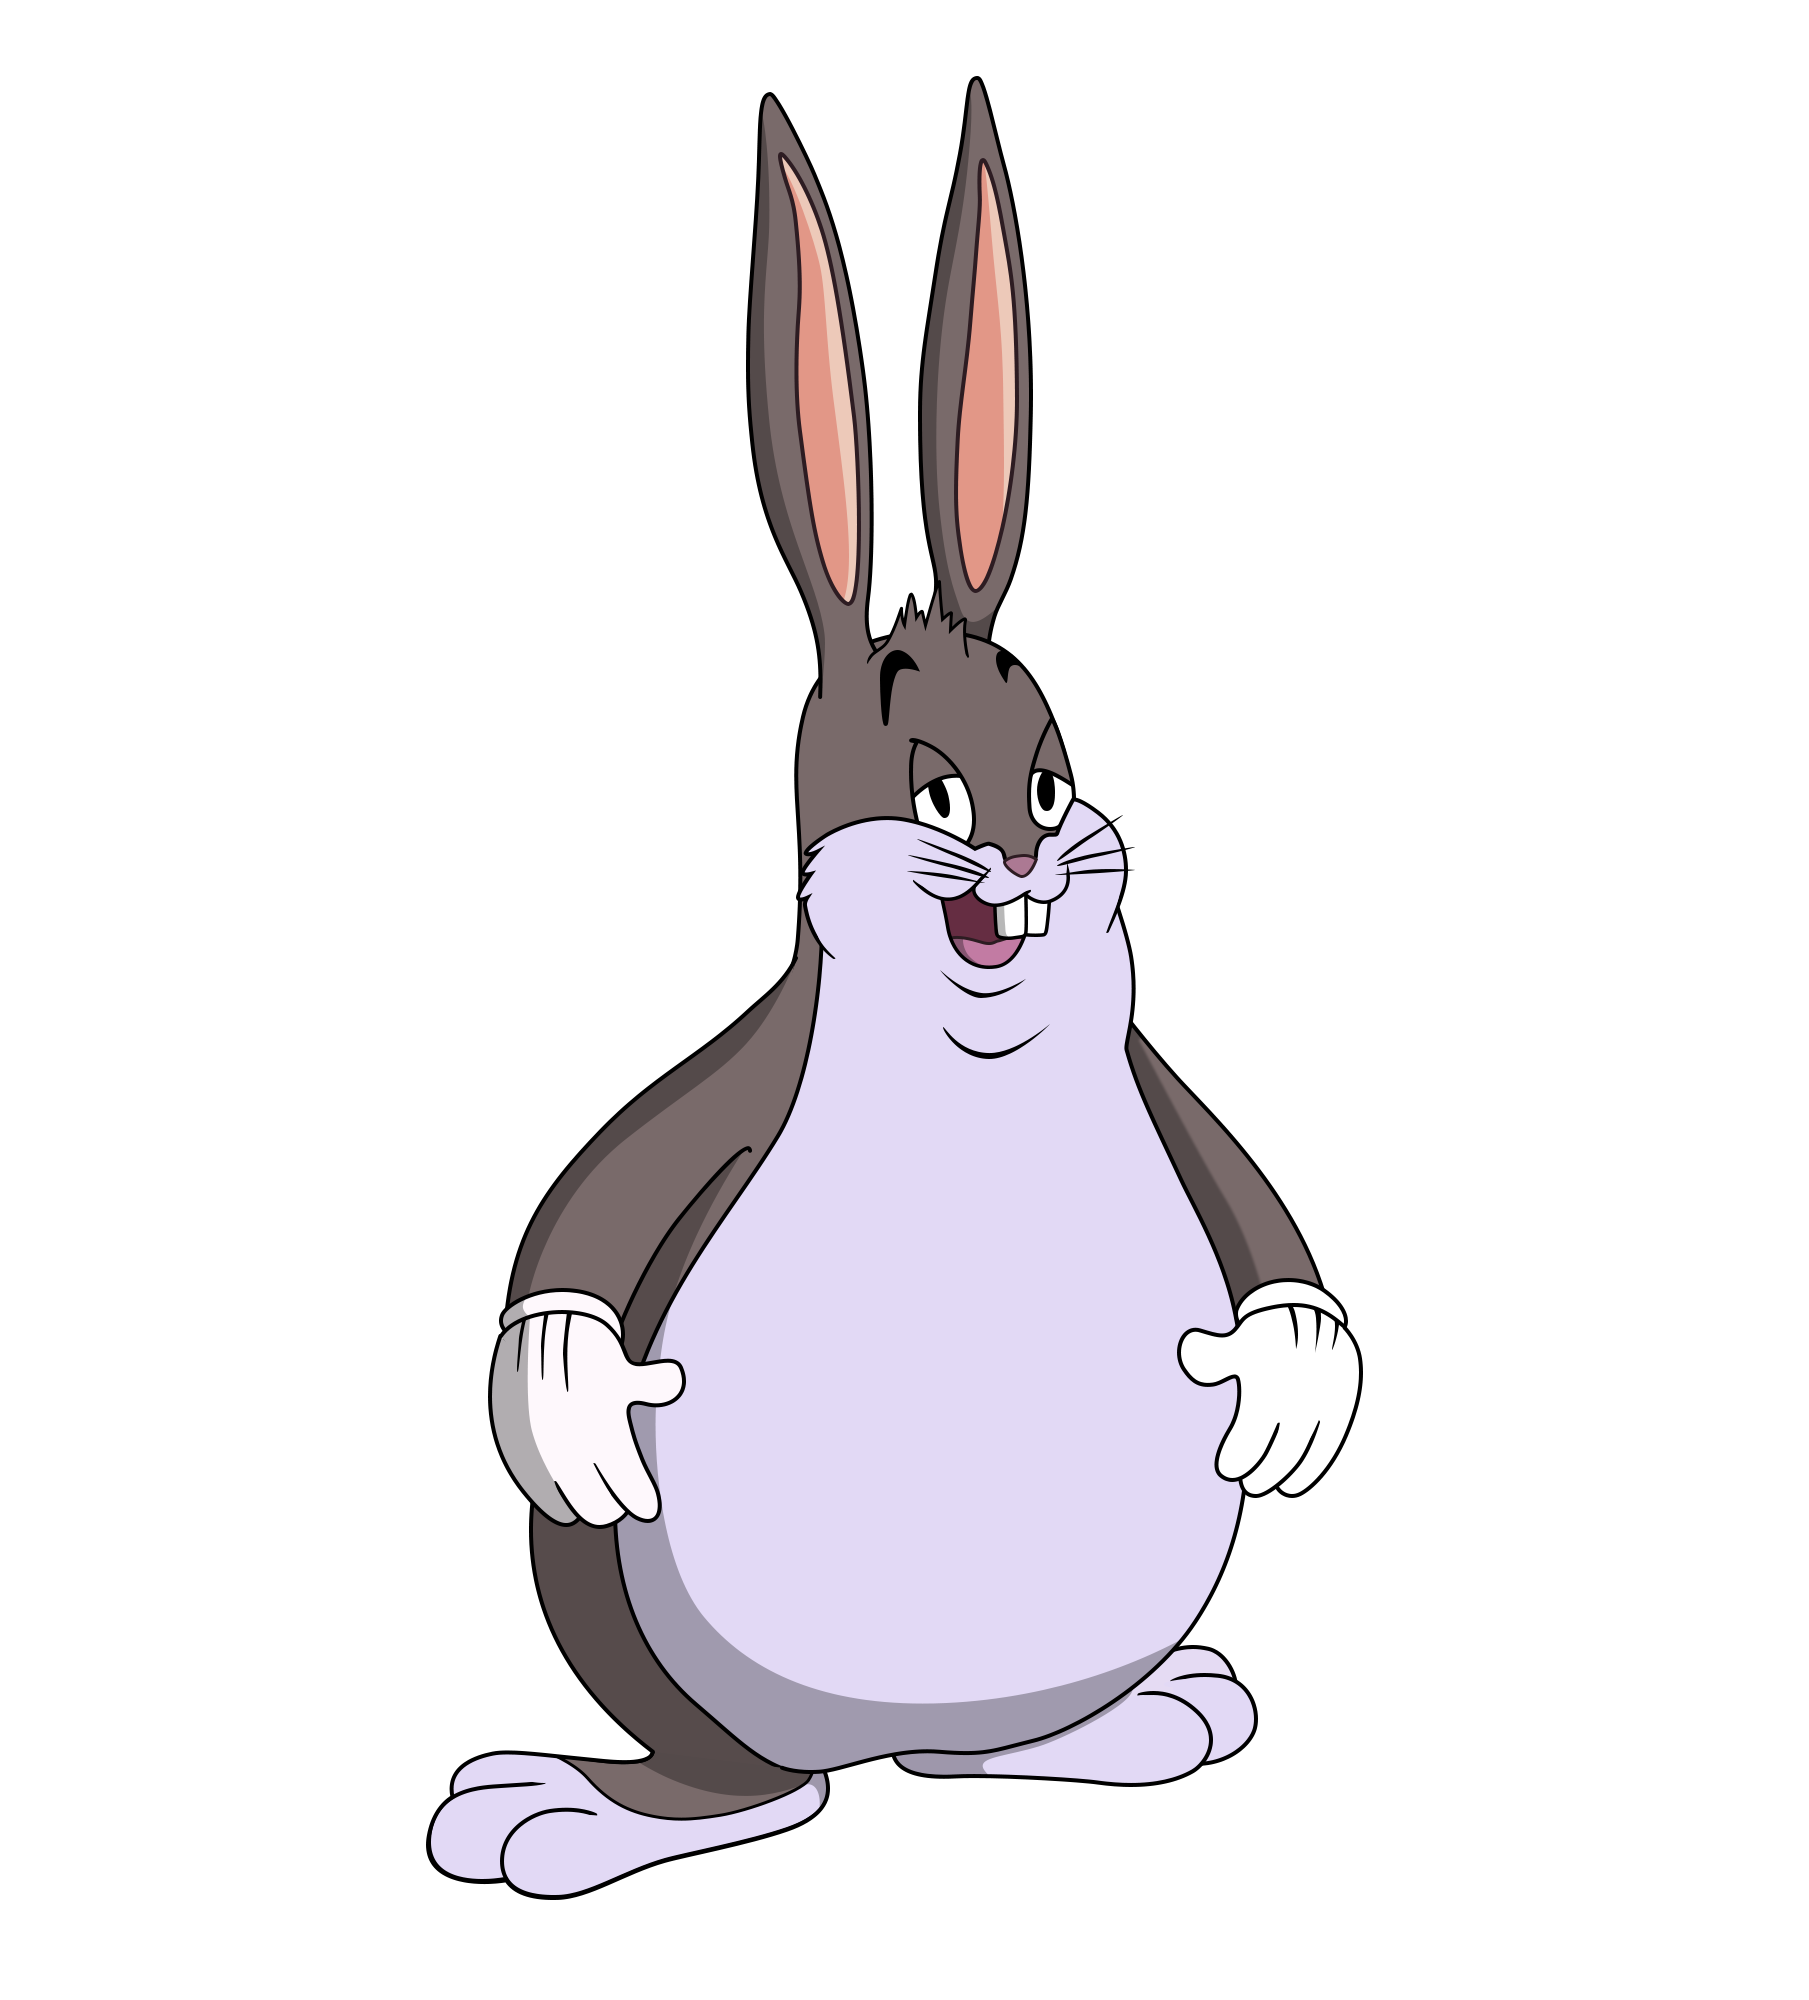
\includegraphics[height=8cm]{img/chungus.png}}

\begin{document}

\maketitle

\begin{frame}{Learning objectives this tutorial}
\begin{itemize}
\item Talk about the definition ``computably enumerable set''.
\item Conclude that it doesn't really matter which definition we use!
\end{itemize}
\end{frame}

\begin{frame}{Computably Enumerable Sets}
Assignment 1 recall time! My sincerest apologies.

\begin{figure}
    \centering
    
\includegraphics[scale=0.3]{img/oh.png}
\end{figure}


\textbf{Question}: What was our original informal definition of a CE set, from the first assignment? 

\pause

\textbf{Ans}: A set $M \subseteq \N$ is CE if we can write a computer program that outputs the elements of $M$ in a list.
\end{frame}

\begin{frame}{Computably Enumerable Sets}
A set $M \subseteq \N$ is CE if we can write a computer program that outputs the elements of $M$ in a list.

But how do we ``output'' an infinite set? We can write a computer program that prints $2, 4, 6, 8, \ldots$, but a computer will never finish outputting all the even numbers!

\pause

What we mean here is: given any $m \in M$, the computer program will eventually print out $m$.\footnote{It is not necessary that we print the numbers in increasing order! So $2, 6, 4, 8, \ldots$ is also a valid way to enumerate the evens.}
\end{frame}

\begin{frame}[fragile]{Computably Enumerable Sets}
\textbf{Task}: Show that the set of prime numbers $P$ is CE.\footnote{Recall that a natural number $n$ is prime if and only if $n \neq 1$, and its only divisors are $1$ and $n$} In other words, write a program\footnote{In Python, C, Minecraft, ChungusCode, or whatever language you choose!} that prints out the prime numbers.

\pause

\textbf{Ans}:

\vspace{3mm}

\begin{minipage}{0.6\textwidth}
\begin{verbatim}
i = 2
while True:
  is_prime = True
  for j in range(i):
    if i % j == 0:
      is_prime = False
  if is_prime:
    print(i)
  i += 1
\end{verbatim}
\end{minipage}
\begin{minipage}{0.3\textwidth}
Output:
\begin{verbatim}
2
3
5
7
11
13
...
\end{verbatim}
\end{minipage}
\end{frame}

\begin{frame}{Formal definition of CE set}

Recall in Lecture 3 that we built up a set of functions called the ``partial recursive'' functions, in an attempt to mimicking what a computer can do.

\vspace{2mm}
\pause

A partial recursive function $f: \N \to \N$ is said to be \textit{total} if $f(n)$ is defined for all $n \in \N$. Some synonyms for ``total'' functions are ``\textit{total recursive}'' and ``\textit{\textbf{computable}}''. 

\vspace{2mm}
\pause

All primitive recursive functions are recursive and defined for all natural numbers, so they are all computable! But some computable functions are not primitive recursive.

\vspace{2mm}
\pause

\color{red}

\textbf{Correction to last week's tutorial}: Again, we lied to you! 
\begin{itemize}
    \item Last week's definition: A computable set is a set whose characterstic function\footnote{Recall: If $S \subseteq \N$ is a set, the characteristic function of $S$ is defined as $\chi_S(n) = \begin{cases}
    1 & n \in \N\\
    0 & n \notin \N.
    \end{cases}$} is primitive recursive. 
    \item This week's definition: A computable set is a set whose characterstic function is computable (as  we have just defined). 
\end{itemize}

\end{frame}


\begin{frame}{Formal definition of CE set}

Now we will present the formal definition of a CE set (from Lecture 3 also).

\textbf{Definition}: A set $S \subseteq \N$ is \textbf{CE} when one of the following holds:
\begin{itemize}
    \item $S = \emptyset$;
    \item $S$ is the range of a computable function $f$. That is,
    $$S = \{f(n): n \in \N\}.$$
\end{itemize}

\textbf{Write this down!!}

\pause

\textbf{Question}: What does the Church-Turing Thesis say?

\pause

\textbf{Ans}: The Church-Turing Thesis says that a function $f$ is ``intuitively computable'' iff it is total recursive (iff it is Turing computable, iff it is URM computable, etc).

\pause

\textbf{Task}: Let $P$ be the set of primes. Show that $P$ is CE according to the above definition, by showing that $f(n) = \text{the $n$th prime number}$ is computable using the CT Thesis.

\end{frame}

\begin{frame}[fragile]{Formal definition of CE set}

\textbf{Task}: Let $P$ be the set of primes. Show that $P$ is CE according to the above definition, by showing that $f(n) = \text{the $n$th prime number}$ is computable using the CT Thesis.

\vspace{2mm}

\textbf{Ans}: Define $f: \N \to \N$, $f(n) = \text{the $n$th prime number}$. $f$ is intuitively computable, because we can write the following program to compute $f$:

\begin{minipage}{0.36\textwidth}
\begin{verbatim}
def is_prime(i):
  for j in range(i):
    if i % j == 0:
      return False
  return True
\end{verbatim}
\end{minipage}
\begin{minipage}{0.36\textwidth}
\begin{verbatim}
def f(n):
    # the 0th prime is 2!
    prime_count = -1
    i = 2
    while True:
      if (is_prime(i)):
        prime_count += 1
      if (prime_count == n):
        return i
      i += 1
\end{verbatim}
\end{minipage}

By the CT Thesis, $f$ is computable (in the recursive sense). So $P$, which is the range of $f$, is a CE set.

\end{frame}



\begin{frame}{Equivalent definition 2}

We will now prove the following:
$$\text{$S$ is CE} \Leftrightarrow \text{$S$ is the domain of a partial recursive function}.$$

Recall: if $g(x, y)$ is partial recursive, then so is
$$f(x) = \min\{y: g(x, y) = 0\}.$$

\pause

\textbf{Task}: Show that $\emptyset$ is the domain of a partial recursive function. In other words, come up with a partial recursive function that is defined \textit{nowhere}!

\pause

\textbf{Ans}: Define $g(x, y) = 1$ for all $x, y$. Since intuitively $g$ is computable (just return $1$ regardless of input), $g$ is computable. As computable functions are (partial) recursive,
$$f(x) = \min\{y: g(x, y) = 0\}$$
is also partial recursive. But $f(x)$ is undefined for any $x \in \N$! Thus $\text{domain}(f) = \emptyset$.

\end{frame}


\begin{frame}{Equivalent definition 2}

$$\text{$S$ is CE} \Rightarrow \text{$S$ is the domain of a partial recursive function}.$$

Let's prove the theorem! Recall that a set $S$ is formally CE if it satisfied one of the following:
\begin{itemize}
    \item $S = \emptyset$.
    \item $S = \text{range}(f)$ for some computable $f$.
\end{itemize}

\textbf{Task:} Show that if $S$ is formally CE, then $S$ is the domain of a partial recursive function.

\pause

\textbf{Ans}: Suppose $S$ is CE. We have two cases:
\begin{itemize}
    \item $S = \emptyset$: On the previous slide, we've proven that $\emptyset$ is the domain of a partial recursive function.
    \item $S = \text{range}(f)$ where $f$ is computable. Define the computable function $g(x, y) = |x - f(y)|$ (so $g(x, y) = 0$ iff $x = f(y)$). Then the function
    $$h(x) = \min\{x: g(x, y) = 0\}$$
    is partial recursive. $h$'s domain is precisely the range of $f$!
\end{itemize}

\end{frame}


\begin{frame}[fragile]{Equivalent definition 2}

$$\text{$S$ is CE} \Leftrightarrow \text{$S$ is the domain of a partial recursive function}.$$

What about the other direction? (It's hard!)

\pause

Let $S = \text{domain}(f)$, where $f$ is partial recursive. If $S = \emptyset$ then $S$ is CE and we're done, so suppose $S \neq \emptyset$. Since $S$ is nonempty, choose some $s \in S$.

We may define the following computable function $g$:
\begin{verbatim}
def g(x, s):
  try to compute f(x) for s steps
  if f(x) returns within s steps:
    return x
  else: 
    return s
\end{verbatim}

\textbf{Task}: Show that the range of $g$ is indeed $S$.

\end{frame}

\begin{frame}[fragile]{Equivalent definition 2}
So we've proven the following!

$$\text{$S$ is CE} \Leftrightarrow \text{$S$ is the domain of a partial recursive function}.$$

\pause

It also turns out that 
$$\text{$S$ is CE} \Leftrightarrow \text{$S$ is the range of a partial recursive function}.$$

But we don't have time to prove this! :(
\pause

This equivalence of definitions is called the \textbf{Normal Form Theorem}.

\end{frame}







\end{document}